\documentclass{article}
\usepackage{graphicx} % For including images
\usepackage{titling}  % For custom title page
\usepackage{circuitikz}
\usepackage{amsmath}
\usepackage{amssymb}
\usepackage{booktabs,tabu}
\usepackage[all, cmtip]{xy}
\newcommand{\ohm}{\Omega}
% Set up title and author
\title{Experiment 6: Sampling}
\author{Samyak Sheersh,Souhardya Bose,Aryam Shankar}
\date{21 October 2024}
\newcommand{\subtitle}[1]{%
  \posttitle{%
    \par\end{center}
    \begin{center}\large#1\end{center}
    \vskip0.5em}%
}

\begin{document}

% Custom title page
\begin{titlepage}
    \centering
    
\includegraphics[width=0.2\textwidth]{KGP_logo.png}\par\vspace{1cm}
    {\scshape\LARGE Department of Electronics and Electrical Communication Engineering, IIT Kharagpur\par}
    \vspace{1cm}
    {\huge\bfseries Experiment 7: Analog to Digital conversion\par}
    \vspace{1.5cm}
    {\Large\itshape Samyak Sheersh,Souhardya Bose,Aryam Shankar\par}
    \vfill
    % Identifying information at the bottom
    {\large Roll Numbers: 22EC30045, 21EE10097, 22EC3FP37\par}
    {\large Group Number: 12\par}
    \vfill
    {\large 26 October 2024\par}
\end{titlepage}


\section{Introduction}
\subsection{Objectives}
\begin{enumerate}
  \item To quantize the voltages after sampling.
\end{enumerate}
\section{Instruments and Materials Used}
\begin{enumerate}
  \item RIGOL Signal Generator
  \item ScientiFIC SMO10C Digital Signal Oscilloscope
  \item +12V, -12V DC source and ground
  \item Resistors
  \item Capacitors
  \item Diodes
  \item Breadboard
  \item Connecting wires
  \item JFET
  \item ADC 0802
\end{enumerate}
\section{Theory}
In the previous experiment, we sampled the signal which discretized it in the time domain. However, the values of the signal were still taking values in a continuum. Thus to process it using a discrete setup, we would need to obtain an output which only takes up finite values i.e. we need to discretise the voltage levels. 
\clearpage
\section{Circuit Diagram}
\begin{figure}[!ht]
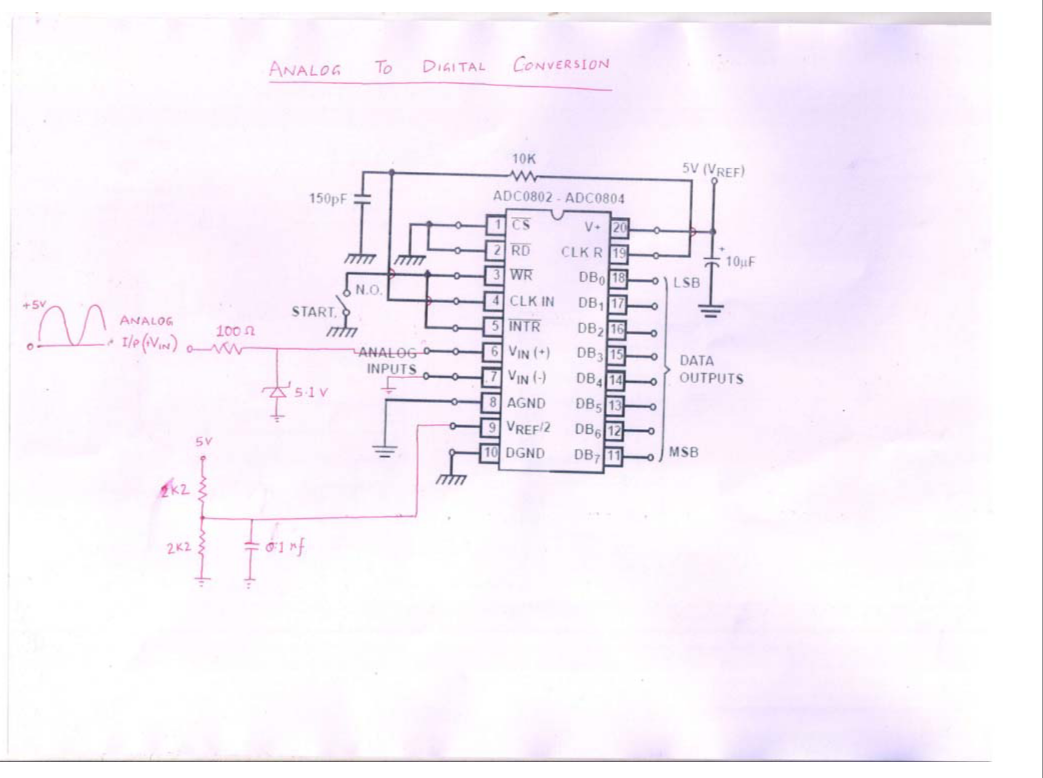
\includegraphics[width=\textwidth]{Circuit.png}
\caption{Circuit for quantizing the sample and hold signal from Expt 6.}
\label{fig:cir}
\end{figure}
\clearpage
\section{Observations and Results}
\begin{figure}[!ht]
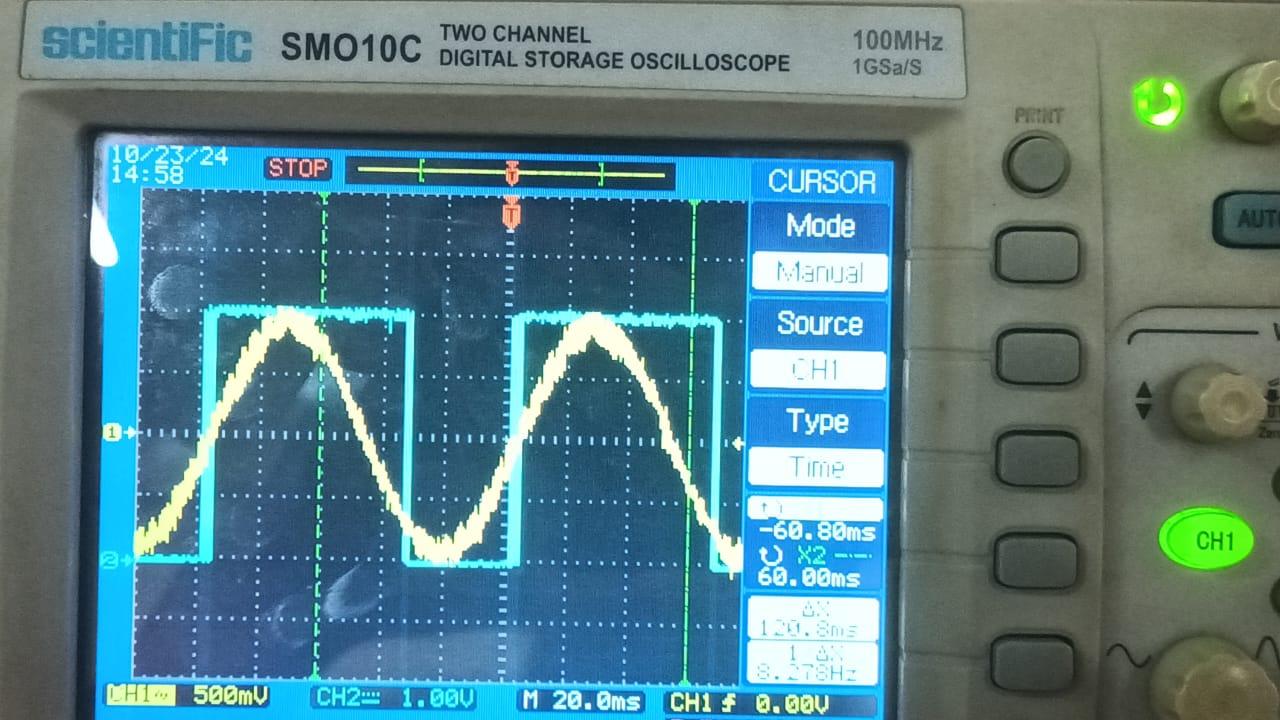
\includegraphics[width=\textwidth]{Sample_and_hold.jpeg}
\caption{Sample and hold signal, and the Most significant bit(MSB) @ 10Hz}
\label{fig:MSB}
\end{figure}
\section{Discussion}
\subsection{Samyak Sheersh, 22EC30045}
\begin{enumerate}
  \item The IC we used for Analog to Digital Conversion (ADC 8202) was an 8-bit converter with reference voltage was from 0 to 5V. 
  \item We had input the signal with $V_{pp}=2V$ with an offset of $V_{dc}=3V$ such that the signal never goes to negative voltage. Thus, the actual variation we get is from $V_{min}=1V$ to $V_{max}=5V$.
  \item Since it represents the voltages using 8 bits, where $00000000$ would correspond to $0V$ and $11111111$ would correspond to $5V$. Thus the MSB would be on whenever the reference signal goes above 2.5V, as we can clearly see from the DSO output
  \item We could also see (by using LED pins) that the MSB was changing the slowest of them all, while the LSB had the highest frequency, which is expected since even changes of $\frac{5}{2^{8}-1}\approx 0.02V$ would lead to a change in the level that the sample is assigned to.  
\end{enumerate}
\end{document}

